\chapter{Antecedentes}
En este capítulo se presentan los antecedentes y conceptos teóricos necesarios para entender este trabajo, y se divide en dos secciones principales. La primera, presenta los conceptos de control de flujo de información, mientras que la segunda, presenta los conceptos de inferencia de tipos.

\section{Control de flujo de información} \label{controlflujo}
Los lenguajes con tipado de seguridad para el control del flujo de la información clasifican los valores de un programa con respecto a sus niveles de confidencialidad, expresado mediante un retículo\footnote{Un orden parcial, donde todo par de elementos tiene un único supremo e ínfimo} (\emph{lattice}) de etiquetas de seguridad. Por ejemplo, con el retículo de dos niveles de seguridad \texttt{L} $\sqsubseteq$ \texttt{H} se puede distinguir entre valores públicos o de baja confidencialidad (\texttt{L}) y valores privados o de alta confidencialidad (\texttt{H}). Un sistema de tipos con control de flujo asegura de forma estática el cumplimiento de la propiedad de no-interferencia~\cite{noninterference}, esto es, que la información confidencial no fluya directa o indirectamente hacia canales públicos~\cite{volpanoAl:S96}.

En el siguiente ejemplo se muestra un código anotado con niveles de seguridad, en donde el parámetro \texttt{guess} y el retorno del método se declaran de baja confidencialidad, y el parámetro \texttt{password} se declara de alta confidencialidad.

\begin{ej} \ \\
  \normalfont
  \label{ej2-1}
\begin{lstlisting}
  bool@L login(String@L guess, String@H password) {
    return password == guess;
  }
\end{lstlisting}
\end{ej}

En el ejemplo \ref{ej2-1} ocurrió un flujo explícito, debido a que un observador público puede obtener información del parámetro confidencial \texttt{password} observando las salidas del programa, lo que no ocurriría si \texttt{login} declara un retorno de tipo \texttt{bool@H}.

Un flujo explícito significa una infracción a no-interferencia. Para su detección, los lenguajes de seguridad poseen distintas reglas que relacionan los niveles de seguridad involucrados. En una instrucción de asignación \texttt{x = y}, se dice que el nivel de seguridad de \texttt{y} debe ser igual o menor que el nivel de seguridad de \texttt{x}. En una instrucción de retorno \texttt{return y}, se dice que el nivel de seguridad de \texttt{y} debe ser igual o menor que el nivel de seguridad declarado como retorno del método. En el ejemplo \ref{ej2-1}, el nivel de seguridad de la comparación es \texttt{H}, debido a la propagación del nivel de seguridad de \texttt{password} en la operación de comparación. Esto es mayor que el nivel de seguridad de retorno \texttt{L}.

En el siguiente ejemplo se introduce una variable global al ejemplo \ref{ej2-1} para almacenar el valor de retorno, y se cambia el tipo de retorno de la función por \texttt{void}. Además, se considera que los valores literales son de baja confidencialidad.

\begin{ej} \ \\
  \normalfont
  \label{ej2-12}
\begin{lstlisting}
  String@L ret = "";
  void login(String@L guess, String@H password) {
    if (password == guess) ret = "Login successful";
    else ret = "Login failed";
  }
\end{lstlisting}
\end{ej}

En el ejemplo \ref{ej2-12} ocurrió un flujo implícito, debido a que un observador público puede obtener información del parámetro confidencial \texttt{password} observando cambios en el valor que contiene la variable \texttt{ret}, mediante el control de flujo del programa.

Un flujo implícito también significa una infracción a no-interferencia. Es posible detectar un flujo implícito considerando que las instrucciones de retorno y asignación de valores de baja confidencialidad, ocurren en un contexto de alta confidencialidad, determinado por la condición de la instrucción \texttt{if}. Para considerar el contexto de ejecución de una instrucción en las reglas del sistema de tipos, se utiliza el concepto de \emph{program counter} (\texttt{pc}) para seguridad~\cite{pc}. Así, en el ejemplo \ref{ej2-12} las instrucciones de asignación son inválidas, debido a que asignan valores de baja confidencialidad cuando el \texttt{pc} tiene un valor de alta confidencialidad.

A pesar de que no-interferencia es una propiedad atractiva para la especificación de sistemas seguros, se considera muy estricta en la práctica, debido a que impide que la información confidencial tenga cualquier tipo de influencia en una salida observable de un programa. En efecto, queremos que el programa de \texttt{login} sea aceptado a pesar de no cumplir con la propiedad, pues de otra forma no tendríamos cómo realizar la autenticación.

Para solucionar este problema, los lenguajes de seguridad adicionan mecanismos de desclasificación que disminuyen el nivel de seguridad de un valor confidencial, implementados de diferentes formas~\cite{sabelfeldSands:JCS09}. Una de ellas, por ejemplo en Jif~\cite{jif} es usar un operador \texttt{declassify}, que desclasifica un valor de alta confidencialidad retornando un valor de baja confidencialidad. En el ejemplo \ref{ej2-2}, se utiliza para desclasificar el resultado de la operación de comparación.
\clearpage
\begin{ej} \ \\
  \normalfont
  \label{ej2-2}
\begin{lstlisting}
  String@L login(String@L guess, String@H password) {
    if (declassify(password == guess)) return "Login Successful";
    else return "Login failed";
  }
\end{lstlisting}
\end{ej}


A pesar de que este programa no cumple con no-interferencia, no representa una amenaza de seguridad, debido a que el resultado de la operación de comparación es negligible con respecto al parámetro privado \texttt{password}. Sin embargo, usos arbitrarios del operador \texttt{declassify} pueden resultar en serias fugas de información. Por ejemplo, \texttt{declassify(password)} puede dar conocimiento absoluto sobre el valor de la variable a un observador público.

Varios mecanismos se han explorado para controlar el uso de desclasificación, y poder asegurar además una propiedad de seguridad para el programa~\cite{sabelfeldSands:JCS09}. En esta dirección, Cruz et al.~\cite{cruzAl:ecoop2017} recientemente propusieron la desclasificación basada en tipos como un mecanismo de desclasificación que conecta la abstracción de tipos con una forma controlada de desclasificación, en una manera intuitiva y expresiva, proveyendo garantías formales sobre la seguridad del programa.

En la desclasificación basada en tipos, los tipos tienen dos facetas; la faceta privada, que refleja el tipo de implementación, y la faceta pública, que refleja las operaciones de desclasificación sobre los valores de dicho tipo. Por ejemplo, el tipo $\mathtt{StringEq} \triangleq [\mathtt{eq} : \mathtt{String} \rightarrow \mathtt{Bool}]$\footnote{La notación $t_1\rightarrow t_2$ corresponde al tipo de una función con parámetro de tipo $t_1$ y retorno de tipo $t_2$} autoriza la operación \texttt{eq} sobre un \texttt{String}. Entonces se puede usar el tipo de dos facetas \texttt{String<StringEq} para controlar la operación de desclasificación de la igualdad sobre \texttt{password}, lo que se muestra en el ejemplo \ref{ej2-3}
\begin{ej} \ \\
  \normalfont
  \label{ej2-3}
\begin{lstlisting}
  String<String login(String<String guess, String<StringEq password) {
  	if (password.eq(guess)) return "Login successful";
  	else return "Login failed";
  }
\end{lstlisting}
\end{ej}


En la desclasificación basada en tipos, se cumple que la faceta privada es subtipo de la faceta pública. En el ejemplo \ref{ej2-3}, \texttt{String} es subtipo de \texttt{StringEq}, relación que se escribe como \texttt{String <: StringEq}. Los tipos que cumplen con esta relación se denominan bien formados (\emph{well-formed}).

Al igual que en tipado de seguridad de dos o más niveles, las facetas de la desclasificación basada en tipos forman un retículo con relaciones de subtipos, lo que se ejemplifica en la figura \ref{l1}, donde \texttt{StringEq} $\triangleq [\mathtt{eq} : \mathtt{String} \rightarrow \mathtt{Bool}]$ y \texttt{StringEqLength} $\triangleq [\mathtt{eq} : \mathtt{String} \rightarrow \mathtt{Bool}, \mathtt{length} : \mathtt{Unit} \rightarrow \mathtt{Int}]$.
\clearpage
	\begin{figure}[ht]
		\centering
		\begin{tikzpicture}[node distance=2.3cm]
			\node(Top) 												{\texttt{Top}};
			\node(StringEq)		[below right of=Top]			{\texttt{StringEq}};
			\node(StringEqLength)      [below of=StringEq]       {\texttt{StringEqLength}};
			\node(String)				[below of=StringEqLength]       {\texttt{String}};
			\node(int)					[below left of=Top] 			{\texttt{int}};
			\draw(Top)      -- (StringEq);
			\draw(Top)      -- (int);
			\draw(StringEq)      -- (StringEqLength);
			\draw(StringEqLength)      -- (String);
		\end{tikzpicture}
		\caption{retículo de subtipos}
    \label{l1}
	\end{figure}

Si la faceta pública coincide con la faceta privada, toda operación sobre el valor estará autorizada. Cuando esto sucede, se refiere usualmente a la faceta pública con \texttt{Bot}, por encontrarse siempre en la parte inferior del retículo. Cuando se quiere referir a una faceta pública vacía o que no autoriza ninguna operación, se usa \texttt{Top}, por encontrarse en la parte superior del retículo.

Los métodos declarados en la faceta pública también poseen tipos de dos facetas en sus firmas. Así, el tipo \texttt{StringEq} visto anteriormente se define como $\mathtt{StringEq} \triangleq [\mathtt{eq} : \mathtt{String<String} \rightarrow \mathtt{Bool<Bool}]$.

Existen dos reglas principales para comprobar que un programa con tipos de dos facetas se encuentra bien tipado. Consideremos el siguiente ejemplo, en donde $\mathtt{StringHashEq} \triangleq [\mathtt{hash} : \mathtt{Unit<Unit} \rightarrow \mathtt{String<StringEq}]$.

\begin{ej} \ \\
  \normalfont
  \label{ej2-6}
\begin{lstlisting}
  String<StringEq getHash(String<StringHashEq password) {
  	return password.hash();
  }
\end{lstlisting}
\end{ej}

En el ejemplo \ref{ej2-6}, el valor de retorno de la invocación al método \texttt{hash} sobre el parámetro \texttt{password}, tiene faceta pública \texttt{StringEq}, debido a que fue declarado de esta forma en la faceta pública \texttt{StringHashEq}. A esta regla se le llama \texttt{TmD}.

Ahora consideremos el siguiente ejemplo, en donde se cambia la faceta pública del parámetro \texttt{password} del ejemplo \ref{ej2-6} por \texttt{StringEq}.
\clearpage
\begin{ej} \ \\
  \normalfont
  \label{ej2-7}
\begin{lstlisting}
  String<Top getHash(String<StringEq password) {
  	return password.hash();
  }
\end{lstlisting}
\end{ej}

En el ejemplo \ref{ej2-7} se realiza una invocación al método \texttt{hash} sobre el parámetro \texttt{password}, que declara una faceta pública que no autoriza la operación. Cuando esto sucede, la faceta pública de retorno de la invocación es \texttt{Top}. A esta regla se le llama \texttt{TmH}.

La propiedad de seguridad que se demuestra para el sistema de tipos de la desclasificación basada en tipos es una forma de no-interferencia con políticas de desclasificación, denominada no-interferencia relajada (\emph{Relaxed noninterference}). Un lenguaje de seguridad que cumple con esta propiedad, garantiza que la información confidencial solo puede fluir hacia canales públicos de forma controlada, por medio de las políticas de desclasificación.

\section{Inferencia de tipos} \label{inference}
En la sección anterior se revisaron los conceptos relacionados a control de flujo de información, que sirven para comprender el trabajo de la desclasificación basada en tipos. En esta sección se revisan los conceptos relacionados a inferencia de tipos, necesarios para comprender la propuesta de esta memoria.

La inferencia de tipos es el proceso de determinar el tipo de las expresiones en un programa, basado en cómo son usadas. Tener un mecanismo de inferencia en un lenguaje de programación puede ser muy útil, debido a que da la posibilidad al programador de omitir las declaraciones de tipo para algunos identificadores, y mantener los beneficios de un lenguaje estáticamente tipado.

Para ilustrar los conceptos importantes de inferencia, consideremos un lenguaje sencillo con funciones y operaciones aritméticas sobre enteros, cuya sintaxis se muestra en el siguiente ejemplo.
\vspace{0.8em}
\begin{ej}
  \normalfont
  \label{ej2-8}
\begin{lstlisting}
  let g = (x) => x + 5;
\end{lstlisting}
\end{ej}

En el ejemplo \ref{ej2-8}, se asigna a \texttt{g} una función que retorna la suma entre \texttt{x} y \texttt{5}. Notar que no se anotó el tipo de los identificadores \texttt{g} y \texttt{x}.

En la etapa de tipar un programa (\emph{type checking}), los sistemas de inferencia asignan una variable de tipo a cada expresión sin un tipo conocido, y un tipo concreto\footnote{Un tipo concreto no tiene variables de tipo} (por ejemplo, \texttt{int}) a cada expresión con tipo conocido. Además, generan un conjunto de restricciones que se deben cumplir para que cada expresión esté bien tipada.
\clearpage

Una restricción representa una relación entre dos tipos. Esta relación puede ser de igualdad o de subtipos. El uso de restricciones permite presentar un algoritmo de inferencia de forma modular, como una fase de generación de restricciones, y una fase de resolución de restricciones.

La figura \ref{tabla1} muestra la asignación de tipos a cada una de las expresiones del ejemplo \ref{ej2-8}, y las restricciones que se generan.


\begin{figure}[ht]
  \centering
  \ttfamily
  \begin{tabular}{c c c}
    Expresión & Tipo & Restricciones\\
    \hline
    (x) =>\ x + 5 & X & $\mathtt{X = Y \rightarrow Z}$\\
    x & Y & -\\
    x + 5 & Z & Y = int, Z = int\\
    + & $\mathtt{(int,int) \rightarrow int}$ & -\\
    x & Y & -\\
    5 & int & -\\
  \end{tabular}
  \caption{Etapa de \emph{type checking}}
  \label{tabla1}
\end{figure}

En el ejemplo \ref{ej2-8}, las restricciones generadas representan igualdad entre dos tipos. Las siguientes observaciones permiten derivar el conjunto de restricciones del programa.

\begin{enumerate}
  \item \texttt{(x) =>\ x + 5} es una función anónima que debe tener tipo $\mathtt{Y \rightarrow Z}$, donde \texttt{Y} es el tipo del parámetro y \texttt{Z} es el tipo del cuerpo.
  \item \texttt{x + 5} es una aplicación de la función suma, por lo que su tipo debe coincidir con el tipo de retorno de la función. Además, el tipo de los argumentos debe coincidir con el tipo de los parámetros de la función.
\end{enumerate}

Sintetizando, el conjunto de restricciones generado es el siguiente:

\begin{itemize}
  \item $\mathtt{X = Y \rightarrow Z}$
  \item \texttt{Y = int}
  \item \texttt{Z = int}
\end{itemize}

Una vez que se genera el conjunto de restricciones sobre el programa, se procede a encontrar una solución para las variables de tipo del conjunto. Cuando las restricciones representan relaciones de igualdad, se utiliza el algoritmo de unificación de Damas-Milner~\cite{damasmilner}. Este algoritmo genera un diccionario de variables de tipo a tipos concretos, mediante substituciones. La figura \ref{tabla2} muestra la solución esperada del ejemplo \ref{ej2-8}.

\begin{figure}[ht]
  \centering
  \ttfamily
  \begin{tabular}{c c}
    Variable de tipo & Tipo concreto \\
    \hline
    X & $\mathtt{int \rightarrow int}$  \\
    Y & int \\
    Z & int \\
  \end{tabular}
  \caption{Solución del conjunto de restricciones}
  \label{tabla2}
\end{figure}

\clearpage
Desafortunadamente, el algoritmo de unificación de Damas-Milner no funciona cuando las restricciones representan una relación de subtipos. Consideremos una extensión del lenguaje anterior,  en donde se introducen los tipos \texttt{num} y \texttt{float}, donde se cumple \texttt{float <: num} y \texttt{int <: num}. En el ejemplo \ref{ej2-9} se muestran dos instrucciones de asignación.
\vspace{0.8em}
\begin{ej}
  \normalfont
  \label{ej2-9}
\begin{lstlisting}
  let f = 4;
                ...
                f = 1.5;
\end{lstlisting}
\end{ej}

En el ejemplo \ref{ej2-9}, se asigna la variable de tipo \texttt{X} al identificador \texttt{f}. Las restricciones que se generan para las instrucciones de asignación son:

\begin{itemize}
  \item \texttt{int <: X}
  \item \texttt{float <: X}
\end{itemize}

%Cardelli~\cite{cardelli}

Para resolver este tipo de relaciones, se considera la relación de orden parcial entre los tipos, inducida por la relación de subtipos, que se muestra en la figura \ref{subt1}.

\begin{figure}[ht]
  \centering
  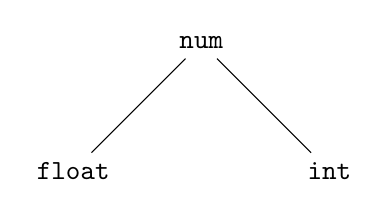
\begin{tikzpicture}[node distance=2.3cm]
    \node(num) 												{\texttt{num}};
    \node(int)		[below right of=num]			{\texttt{int}};
    \node(float)					[below left of=num] 			{\texttt{float}};
    \draw (num)      -- (int);
    \draw (num)      -- (float);
  \end{tikzpicture}
  \caption{Orden parcial entre los tipos}
  \label{subt1}
\end{figure}

Un orden parcial admite las operaciones \texttt{meet} y \texttt{join}, que corresponden a la máxima cota inferior (ínfimo) y a la mínima cota superior (supremo) entre dos tipos, respectivamente. Estas operaciones tienen solución si todo par de tipos en el orden parcial tiene un único supremo e ínfimo, lo que se define como retículo. En la figura \ref{subt1}, se debe agregar el tipo \texttt{Bot} para que el orden parcial sea un retículo.

Luego, se introducen los tipos $\mathtt{t_1 \sqcap t_2}$ y $\mathtt{t_1 \sqcup t_2}$, que representan a las operaciones \texttt{meet} y \texttt{join} entre dos tipos, respectivamente.

En la fase de resolución de restricciones, se aplican las reglas de la proposición \ref{teo1} para generar los tipos correspondientes. Luego, cuando los tipos $\sqcap$ y $\sqcup$ relacionan tipos concretos, se puede materializar la operación sobre el retículo.

%Pese a que Cardelli no considera una inferencia basada en constraints, se puede aplicar este enfoque para la resolución de constraints de subtyping. En efecto, Pottier~\cite{pottier:inria-00073205} y Sekiguchi~\cite{sekiguchi} presentan sistemas de inferencia basados en constraints, con tipos equivalentes a los \texttt{meet} y \texttt{join} de Cardelli.

\begin{prop} \label{teo1} \normalfont Si \texttt{x}, \texttt{y} y \texttt{z} pertenecen a una retículo de subtipos, se cumple lo siguiente: \\
  \begin{itemize}
    \item \texttt{x <: y}, \texttt{x <: z} $\implies$ $\mathtt{x <: y \sqcap z}$
    \item \texttt{y <: x}, \texttt{z <: x} $\implies$ $\mathtt{y \sqcup z <: x}$
  \end{itemize}
\end{prop}

En el ejemplo \ref{ej2-9}, las restricciones generadas se reducen con la aplicación de la proposición \ref{teo1}, lo que da como resultado la restricción $\mathtt{int\sqcup float <: X}$. Como \texttt{int} y \texttt{float} son tipos concretos, se puede materializar la operación \texttt{join}, lo que da como resultado \texttt{num}.

Finalmente, como la restricción \texttt{num <: X} solo admite una solución para \texttt{X}, se resuelve que \texttt{X} tiene tipo \texttt{num}.

\subsection*{Antecedentes adicionales}

\subsubsection*{Relación de subtipos}

En el ejemplo \ref{ej2-9}, la relación de subtipos es nominal. En una relación de subtipos nominal, el retículo de subtipos es definido explícitamente por el programador o el lenguaje de programación. El ejemplo \ref{ej2-10} muestra una declaración explícita de un retículo de subtipos, mediante el uso del \emph{keyword} \texttt{extends}.

\begin{ej} \ \\
  \normalfont
  \label{ej2-10}
\begin{lstlisting}
  class Animal {
    String getName();
  }
  class Duck extends Animal {
    void cuack();
  }
  class Cat extends Animal {
    void miau();
  }
\end{lstlisting}
\end{ej}

Cuando una relación de subtipos es estructural, el retículo de subtipos se define por la forma que tienen los tipos. El ejemplo \ref{ej2-11} muestra la declaración de las clases que definen una relación de subtipos estructural.

\begin{ej} \ \\
  \normalfont
  \label{ej2-11}
\begin{lstlisting}
  class Animal {
    String getName();
  }
  class Duck {
    String getName();
    void cuack();
  }
  class Cat {
    String getName();
    void miau();
  }
\end{lstlisting}
\end{ej}

\subsubsection*{Inferencia de tipos}

%Los tipos $\sqcap$ y $\sqcup$ fueron utilizados por vez primera en un algoritmo de inferencia por Cardelli~\cite{cardelli}.

% Teniendo en cuenta que los distintos sistemas de inferencia propuestos a lo largo del tiempo comparten características, Odersky \textit{et al.}~\cite{odersky} propusieron el framework \texttt{HM(X)}, que entrega un algoritmo de inferencia genérico para un sistema de tipos basado en constraints que cumpla ciertas condiciones.

% Utilizando el framework \texttt{HM(X)}, Pottier y Simonet~\cite{Pottier} presentaron un análisis de control de flujo con inferencia de tipos de seguridad, que hereda todas las buenas propiedades de \texttt{HM(X)}.
